
\begin{frame}{Problématiques en traitement du signal audionumérique}
\begin{center}
\begin{tikzpicture}[mystyle]
\matrix [column sep=10mm,row sep=5mm,ampersand replacement=\&]
{
\node (i1) {\only<1-2>{Son}\only<3-4>{\alert{contrôleurs}}}; \&
\node [terminal] (i2) {p}; \&
\node  (i3) {\only<2>{label}\only<1>{Son}\only<3-4>{\alert{Son}}}; \\
};
\begin{scope}[every path/.style=line]
  \path (i1) -- node [left] {} (i2);
  \path (i2) -- node [right] {} (i3);
\end{scope}
\end{tikzpicture}
\end{center}
\vspace{.8cm}\only<1-3>{
\begin{description}
\item<1>[X-Y]: codage, séparation de sources, \structure{extension de bande}, inpainting, ...
\item<2>[X-y]: recherche d'information
\item<3>[x-Y]: synthèse
\end{description}}
\only<4>{
Pourquoi travailler sur la synthèse sonore ?
\begin{itemize}
\item attrait personnel pour l'inouï
\item challenge
\item en prise avec les avancées actuelles en apprentissage non supervisé
\end{itemize}}
\end{frame}

\begin{frame}{Requis}
\begin{description}
  \item[fidélité]: ne pas produire d'artefacts audibles
  \item[expressivité]: mécanismes de manipulation simples produisant une modification cohérente de la perception du signal résultant
  \item[versatilité]: les conditions de fidélité et d'expressivité sont remplies pour tout signal d'intérêt pour une tâche donnée
\end{description}
\end{frame}

\begin{frame}{\only<1>{Existant}\only<2>{Objectif}}
\begin{tabular}{cc}
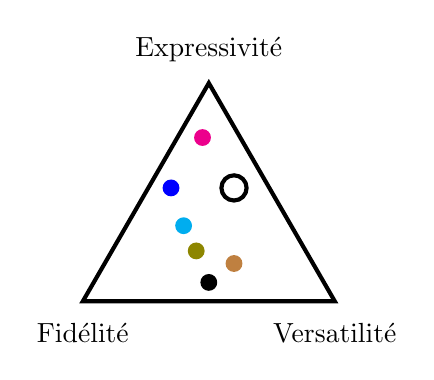
\begin{tikzpicture}[scale=0.8, label distance=1.5mm]
  \coordinate[label=below:Fidélité]  (A) at (0,0);
  \coordinate[label=below:Versatilité] (B) at (4,0);
  \coordinate[label=above:Expressivité] (C) at (2,3.464);
  \draw [line width=1.5pt] (A) -- (B) -- (C) -- cycle;
  \draw [black, fill=black, line width=1.5pt] (2,.3) circle [radius=.1 cm]; % raw
  \draw [olive, fill=olive, line width=1.5pt] (1.8,.8) circle [radius=.1 cm]; % spec
  \draw [brown, fill=brown, line width=1.5pt] (2.4,.6) circle [radius=.1 cm]; % wavelets
  \draw [cyan, fill=cyan, line width=1.5pt] (1.6,1.2) circle [radius=.1 cm]; % sct
  \draw [blue, fill=blue, line width=1.5pt] (1.4,1.8) circle [radius=.1 cm]; % slt
  \draw [magenta, fill=magenta, line width=1.5pt] (1.9,2.6) circle [radius=.1 cm]; % modal
  \only<2>{\draw [black, line width=1.5pt] (2.4,1.8) circle [radius=.2 cm];} % modal
  \end{tikzpicture}

 &

  \begin{tabular}{cl}
    \tikz\draw[black,fill=black] (0,0) circle (.1 cm); & Forme d'onde \\
    \tikz\draw[olive,fill=olive] (0,0) circle (.1 cm); & Spectrogramme \\
    \tikz\draw[brown,fill=brown] (0,0) circle (.1 cm); & Ondelettes \\
    \tikz\draw[cyan,fill=cyan] (0,0) circle (.1 cm); & Sinusoïdes à court terme \\
    \tikz\draw[blue,fill=blue] (0,0) circle (.1 cm); & Sinusoïdes à long terme \\
    \tikz\draw[magenta,fill=magenta] (0,0) circle (.1 cm); & Approches modales
  \end{tabular}
  \end{tabular}
\end{frame}

\begin{frame}{Challenges en traitement du signal}
\newcommand{\blackdot}{\tikz\draw[black,fill=black] (0,0) circle (.1 cm);}
\centering
\begin{block}{La synthèse en audio nécessite d'approcher les challenges suivants}
  \begin{tabular}{c|ccc}
    & fidélité & versatililité & expressivité  \\
  %  \hline
  multirésolution & \blackdot  & \blackdot & \\
  causalité & \blackdot  &  & \blackdot \\
  non linéarité & \blackdot  & \blackdot & \\
  dimensionalité réduite &  & &  \blackdot \\
  contrôle lent &  & &  \blackdot
  \end{tabular}
\end{block}
\end{frame}

\begin{frame}{Schéma fonctionnel}
  \begin{center}
  \structure{IR} \\  \vspace{.2cm}  \begin{tikzpicture}[mystyle]
      \matrix [column sep=10mm,row sep=5mm,ampersand replacement=\&]
      {
      \node (i1) {Son}; \&
      \node [terminal] (i2) {$P$}; \&
      \node [terminal] (i3) {$C$}; \&
      \node (i4) {label}; \\
      };
      \begin{scope}[every path/.style=line]
        \path (i1) -- node [left] {} (i2);
      \path (i2) -- node [above] {$L$} (i3); \path (i3) -- node [right] {} (i4);
      \end{scope}
      \end{tikzpicture}
 \vspace{.4cm} \\  \structure{Synthèse} \\ \vspace{.2cm}
      \begin{tikzpicture}[mystyle]
      \matrix [column sep=10mm,row sep=5mm,ampersand replacement=\&]
      {
      \node (i1) {contrôleurs}; \&
      \node [terminal] (i2) {$c$ \only<2>{\alert{??}}}; \&
      \node [terminal] (i3) {$V$ \only<2>{\alert{??}}}; \&
      \node (i4) {Son}; \\
      };
      \begin{scope}[every path/.style=line]
        \path (i1) -- node [left] {} (i2);
      \path (i2) -- node [above] {$L$} (i3); \path (i3) -- node [right] {} (i4);
      \end{scope}
      \end{tikzpicture}
      \end{center}
      \begin{description}
        \item[$P$]: invariance / stabilité
        \item[$c$]: conditionneur
        \item[$V$]: vocodeur ($\tilde{P^{-1}}$)

      \end{description}
\end{frame}


\begin{frame}{Recherche en cours}
\begin{description}
\item[Vocodeur]: inversion de descripteurs pour la synthèse de scènes sonores respectueuses de la vie privée (Félix Gontier)
\item[conditionneur]: conception interactive en design sonore (Tom Souaille)
\end{description}
\end{frame}

\begin{frame}{Problèmes ouverts}
\begin{itemize}
  \item Spécification des objectifs
  \begin{itemize}
  \item mesures quantitatives de qualité perceptuelles
  \item fonctions de coût perceptivement motivées
  \end{itemize}
\item Synthèse audio neuronale
\begin{itemize}
  \item modèles génératifs adversaires
\item approches basées échantillons
\end{itemize}
\item Opérateur de diffusion d'ondelettes
\begin{itemize}
\item pour le conditionnement
\item pour la synthèse par inversion
\end{itemize}
\end{itemize}
\end{frame}

%


\begin{frame}{Réseau}
\begin{block}{Local}
\begin{itemize}
\item Jean-François Petiot (LS2N)
\item Arnaud Can, Judicaël Picaut, ... (UMRAE, IFSTTAR)
\end{itemize}
\end{block}
\begin{block}{National}
\begin{itemize}
\item Nicolas Misdariis (IRCAM)
\item Catherine Lavandier (U. Cergy)
\end{itemize}
\end{block}
\begin{block}{International}
\begin{itemize}
\item Emmanouil Benetos (QMUL, UK)
\item Vincent Lostanlen (NYU, US)
\item Joakim Andèn (Flatiron Institute, US)
\end{itemize}
\end{block}
\end{frame}

\begin{frame}{Thèmes}
\begin{tikzpicture}[mystyle]
    \matrix [column sep=20mm,row sep=15mm,ampersand replacement=\&]
    {
    \node (imu) {\structure{Musicologie}}; \&
    \node  (ipe) {\structure{Perception}}; \&
    \node  (id) {\structure{Design}}; \\
    \node [align=center](ima) {\structure{Maths} \\ \structure{Appli}}; \&
    \node [terminal,align=center] (its) {Traitement \\du signal\\ audio}; \&
    \node  (iph) {\structure{Acoustique}}; \\
    \node  {}; \&
    \node  (ii) {\structure{Informatique}}; \&
    \node   {}; \\
    };
  \end{tikzpicture}
\end{frame}

\begin{frame}{\only<1>{Thèmes}\only<9>{Un travail en interdisciplinarité} \only<2>{France Télécom R\&D (2001-04)}\only<3>{Bx (2004-06)}\only<4>{Uvic (2006-07)}\only<5>{McGill (2007-08)}\only<6>{Télécom (2008-09)}\only<7>{Ircam (2009-13)}\only<8>{Ls2n (2013-19)}}
  \begin{tikzpicture}[mystyle]
      \matrix [column sep=20mm,row sep=15mm,ampersand replacement=\&]
      {
      \node (imu) {\structure{Musicologie}}; \&
      \node  (ipe) {\structure{Perception}}; \&
      \node  (id) {\structure{Design}}; \\
      \node [align=center](ima) {\structure{Maths} \\ \structure{Appli}}; \&
      \node [terminal,align=center] (its) {Traitement \\du signal\\ audio}; \&
      \node  (iph) {\structure{Acoustique}}; \\
      \node  {}; \&
      \node  (ii) {\structure{Informatique}}; \&
      \node   {}; \\
      };
      \begin{scope}[every path/.style=line, font=\scriptsize]
        \path (ima) -- node [above] {\only<7>{A. Cont}\only<6>{R. Badeau} \only<1>{E. Benetos}} (its);
            \path (ima) -- node [below] {\only<6>{G. Richard}\only<1>{J. Andèn}} (its);
        \path (imu) -- node [right] {\only<3>{M. Robine} \only<8>{G. Lafay} \only<1>{V. Lostanlen}} (its);
        \path (iph) -- node [above] {\only<2>{JB. Rault} \only<5>{P. Depalle} \only<7>{A. Roebel}\only<8>{JR. Gloaguen}  \only<1>{J. Picaut}} (its);
        \path (iph) -- node [below] {\only<5>{G. Scavone} } (its);
        \path [align=left] (ii) -- node [right] {\only<2-3>{S. Marchand}\only<4>{G. Tzanetakis}\only<6>{S. Essid \\ R. Foucard}\only<7>{M. Rossignol}} (its);
        \path [align=left] (id) -- node [right] {\only<1,8>{\hspace{.3cm}JF. Petiot}\only<1,7>{\\ N. Misdariis}} (its);
        \path [align=left] (ipe) -- node [right] {\only<5>{C. Guastavino}\only<1>{C. Lavandier}\only<1,8>{\\ A. Can}} (its);
        \end{scope}
      \end{tikzpicture}
\end{frame}



    % \begin{frame}{Approche}
    % \begin{center}
    %  \includegraphics[width=.6\columnwidth]{longTerme}
    % \end{center}
    % \begin{description}
    % \item[comprendre] : mesure et qualification de l'environnement sonore et de sa perception
    % \item[innover] :
    % \begin{itemize}
    % \item Andy Hildebrand (Autotune)
    % \item Xavier Serra (Vocaloïd)
    % \end{itemize}
    % \end{description}
    % \end{frame}

% \begin{frame}{Déplacements US}
% \begin{block}{Côte ouest}
% \begin{itemize}
% \item \structure{Jesse Engel}, magenta, Google brain (SFB)
% \item Justin Salamon, audio research group, Adobe research (SFB)
% \end{itemize}
% \end{block}
% \begin{block}{Côte est}
% \begin{itemize}
% \item Juan Pablo Bello, music and audio research group, NYU (NY)
% \item Mounya Elhilali, Laboratory for Computational Audio Perception, Johns Hopkins University (Baltimore)
% \end{itemize}
% \end{block}
% \end{frame}

% \begin{frame}{Contributions}
% \small
% Publications
% \begin{itemize}
% \item \fullcite{lagrangeTaslp06}
% \item \fullcite{lagrangeTaslp08}
% \item \fullcite{lafayhal-01111381}
% \end{itemize}
% Logiciels
% \begin{itemize}
% \item \fullcite{explanes}
% \item \fullcite{simscene}
% \end{itemize}
% \end{frame}
